\section{Multilinguale Spracherkennung}
Die Kernidee der mehrsprachigen Spracherkennung ist bei den verschiedenen Architekturen dieselbe. Die Hidden Layer des Deep Neural Networks können als intelligentes Merkmalsextraktionsmodul betrachtet werden, welches aus mehreren Quellsprachen trainiert wird. Nur die Ausgabeschicht liefert eine direkte Übereinstimmung mit den relevanten Klassen. So lassen sich die Extraktoren für eine Reihe verschiedener Sprachen gemeinsam nutzen. 
Wie im folgenden Kapitel erläutert wird, lässt sich somit besonders das Problem beim Lernen der tiefen neuronalen Netze kompensieren. Diese lassen sich aufgrund ihrer Parameter und dem sogenannten Backpropagation-Algorithmus langsamer trainieren. Ein weiterer Vorteil, den dieser Ansatz bietet ist, dass auch mit Sprachen, die nur einen geringen Satz an markierten Trainingsdaten bieten, erlernt werden können. Indem Elemente anderer Sprachen gemeinsam genutzt und übertragen werden, lässt sich diese Herausforderung lösen. Merkmale, die aus diesen neuronalen Netzen extrahiert werden, lassen sich kombinieren, um so die Erkennungsgenauigkeit zu verbessern {\cite{Yu.2014}}.
\\
Eine gemeinsame Nutzung dieser Elemente wird ermöglicht, indem Phoneme zwischen den Sprachen genutzt werden. Da es zwischen verschiedenen Sprachen gleiche Phoneme gibt, müssen diese nicht neu erlernt werden. Um die genannten Ansätze der Sprachidentifikation sowie die der Spracherkennung zu nutzen, müssen Beziehungen zwischen den akustischen Signalen der Sprachen erkannt werden. Jede Sprache besitzt dabei ihre eigenen Charakteristika, wie bereits hervorging. 
\\
In der Sprachübergreifenden Erkennung gibt es einen Satz aus trainierten sowie schlecht bzw. untrainierten Phonemen, die erkannt werden müssen. Die Töne einer Sprache werden mit einem ähnlichen bzw. dem ähnlichsten trainierten Ton einer anderen Sprache ersetzt. Unbekannte Wörter lassen sich somit aus bekannten Phonemen zusammensetzen und korrekt vorhersagen {\cite{UEBLER200153}}. 
\\
Beim Transfer des Modells wird eine neue Softmax-Ebene angelegt und auf eine bestimmte Sprache trainiert, während das gesamte Netzwerk auf die neue Sprache abgestimmt wird. Die Softmax-Funktion wird hierbei lediglich zur Klassifikation verwendet und sorgt dafür, dass der Output immer in einem gleichen Bereich liegt {\cite{Yu.2014}}. Die Ausgabeknoten dieser Schicht entsprechen den Senonen der Zielsprache. Senonen beschreiben hier lediglich das Betrachten des lautlichen Kontextes der einzelnen Phoneme {\cite{Yu.2014}}. Diese Kontexte können komplex sein, da sie zusätzlich den linken und rechten Ton eines Phonems betrachten {\cite{basic_concepts}}.
\\ 
Ein entsprechende Architektur ist in Abbildung \ref{fig:neue_sprache} illustriert. Sie zeigt die gemeinsam genutzten Schichten, die die Merkmale extrahieren sowie die unterschiedlichen Input-Datensätze der einzelnen Sprachen. Jede Sprache hat ihre eigene Softmax-Ebene. Wird ein neuer Datensatz in das System gegeben, werden nur die sprachspezifische Softmax-Ebene angefügt und trainiert sowie die Hidden Layer angepasst. Andere Softmax-Ebenen bleiben unbeeinflusst \cite{Yu.2014}. Dies ist in Abbildung \ref{fig:neue_sprache} zu sehen. 

\begin{figure*}[h!]
	\centering
	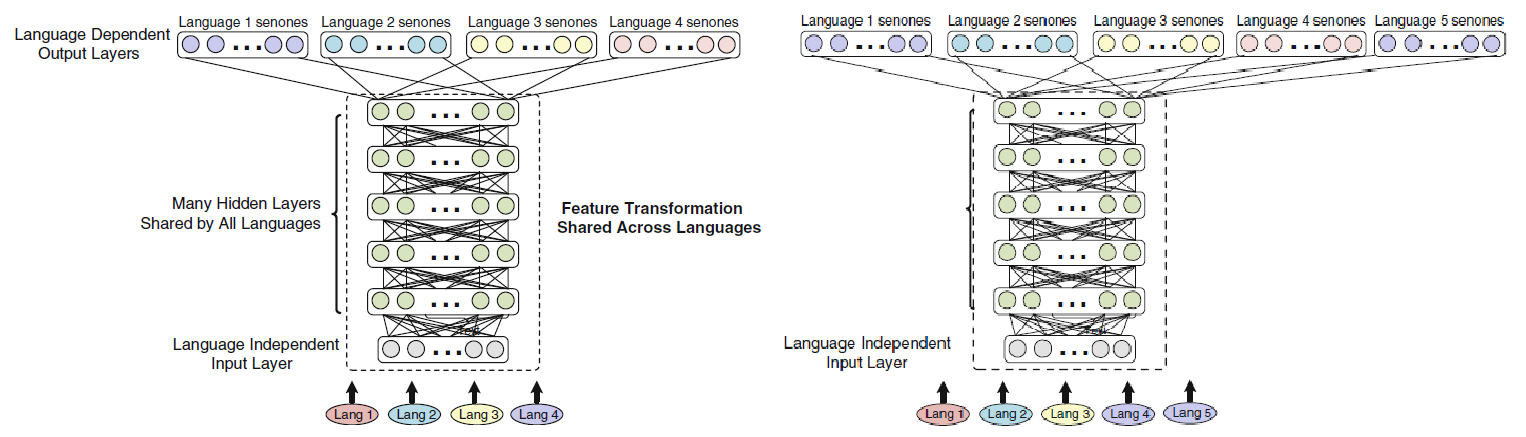
\includegraphics[width=1.0\linewidth]{images/shared_hidden_layer}
	\caption{Hinzufügen einer neuen Sprache  \cite{GonzalezDominguez.2015}} %Generelle
	\label{fig:neue_sprache}
\end{figure*}

Dieser Ansatz bringt eine Verbesserung gegenüber monolingualen Netzwerken. Ein Vergleich eines monolingualen Deep Neural Networks und eines multilingualen Deep Neural Networks ist in Tabelle \ref{table} aufgeführt. Das monolinguale Netzwerk wurde hierbei nur mit jeweils einer der Sprachen französisch, deutsch, spanisch und italienisch trainiert, während das multilinguale System mit allen vier Sprachen trainiert wurde. Dabei wird die prozentuale Wortfehlerrate (Word error rate, WER) angegeben. Es ist zu erkennen, dass das multilinguale System das monolinguale in allen Sprachen übertrifft. Diese Verbesserung ist dem sprachübergreifenden Wissen zuzuschreiben {\cite{Yu.2014}}. Die Steigerungen sind zusätzlich relativ in Prozent angegeben. 

\begin{table*}[h!]
	\begin{tabular}{lllll}
		& FRA             & DEU           & ESP           & ITA             \\
		Test set size (words) & 40k             & 37k           & 18k           & 31k             \\
		Monolingual DNN WER   & 28.1\%          & 24.0\%        & 30.6\%        & 24.3\%          \\
		Multilingual DNN WER  & 27.1\% (-3.6\%) & 22.7 (-5.4\%) & 29.4 (-3.9\%) & 23.5\% (-3.3\%)
	\end{tabular}
	\centering
	\caption{Relative Wortfehlerrate {\cite{Yu.2014}}}
	\label{table}
\end{table*}

In {\cite{6639081}} wurden eine Reihe weiterer Versuche durchgeführt, um die Wirksamkeit eines solchen Systems zu evaluieren. Dabei werden zwei verschiedene Zielsprachen verwendet. Zum einen das amerikanische Englisch, welches phonetisch nahe an den europäischen Sprachen der oben aufgeführten Tabelle liegt und Mandarin-Chinesisch, welches kaum Gemeinsamkeiten zu europäischen Sprachen bietet. Beim Vorhersagen des Gesprochenen kommt die Sprachidentifikation ins Spiel, durch welche Wörter ausgeschlossen werden können, die ebenfalls in Frage kommen, allerdings zum Wortschatz einer anderen Sprache gehören. Es wird hier mit statistischen Modellen gearbeitet, um anzugeben, mit welcher Wahrscheinlichkeit welches Wort vorkommt oder auf ein vorhergehendes folgen könnte. Dabei gibt es verschiedene Lösungsansätze, um das Gesprochene vorherzusagen. Hier wurden bisher tiefe neuronale Netze in Verbindung mit Hidden Markov-Modellen eingesetzt. Diese hybriden Systeme werden in der Literatur untersucht und beschrieben. Ein allerdings leistungsfähigeres Modell bieten die Recurrent Neural Networks. Diese Form von neuronalen Netzen werden heutzutage eingesetzt und erreichen hohe Genauigkeiten {\cite{Yu.2014}}.


\section{Recurrent Neural Networks}
Spracherkennungssysteme erreichen ihre Erkennungsgenauigkeit durch den Einsatz von Recurrent Neural Networks. 
Das Modell dieser Netze erlaubt gerichtete, zyklische Verbindungen zwischen den Neuronen, wodurch es mit einem temporalen Verhalten ausgestattet wird. Recurrent Networks sind somit zum Lernen von Datensequenzen geeignet. Sprachen (kontinuierliche Audiostreams) fallen somit ebenfalls in das Anwendungsgebiet. Diese Form von neuronalen Netzen unterscheiden sich grundlegend von einem Feed Forward Deep Neural Network, da es nicht nur basierend auf Eingaben arbeitet, sondern auch auf interne Zustände zurückgreift. Die internen Zustände speichern die vergangenen Informationen in der zeitlichen Reihenfolge, in welcher diese verarbeitet wurden. Somit ist ein Recurrent Neural Network dynamischer, als ein Deep Neural Network, welches lediglich eine statische Eingabe-Ausgabe-Transformation durchführt \cite{Yu.2014}. In Abbildung \ref{fig:rnn} ist ein vereinfachtes Modell illustriert.

\begin{figure}[H]
	\centering
	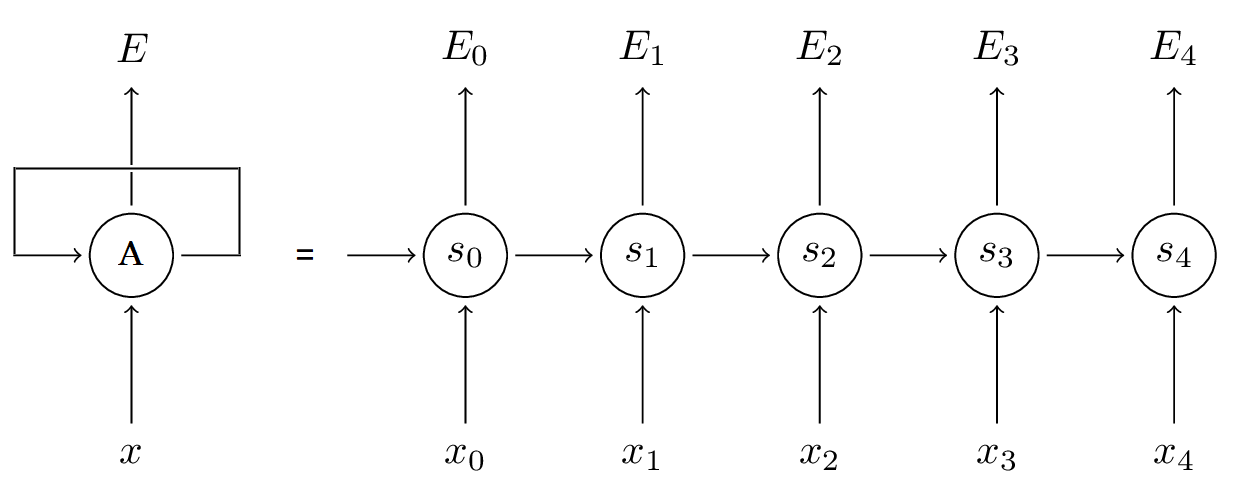
\includegraphics[width=0.8\linewidth]{images/rnn}
	\caption{Modell des Recurrent Neural Network  \cite{GonzalezDominguez.2015}} %Generelle
	\label{fig:rnn}
\end{figure}

Die Abbildung zeigt links ein Netzwerk A, welches über eine Rückkopplung verfügt. Dieses Netzwerk bekommt einen Input x und gibt einen Output bzw. Zustand E zurück. So kann die Information von einem Schritt zum nächsten gelangen. Das ausgerollte Netzwerk wird rechts daneben dargestellt. Es zeigt eine Folge von Iterationen. S bezeichnet den jeweiligen Schritt und E den entsprechenden Hidden State, welcher sich beim Eingeben von Daten zum Zeitpunkt s ergibt. Ein Recurrent Neural Network gibt somit nicht nur den Input an die nächste Iteration, sondern zusätzlich den daraus resultierenden Zustand. Vorhergehende Schritte beeinflussen so die darauf folgenden {\cite{Yu.2014}}. 
\\
Dies führt allerdings zu einem Problem. Dadurch, dass die Zustände immer weiter angepasst werden, verschwindet bzw. verschwimmt im Laufe der Zeit Information. Dies ist als Vanishing Gradient Problem bekannt und ergibt sich dadurch, dass Recurrent Neural Networks nicht in der Lage sind, auf Informationen zurückzugreifen, die weit in der Vergangenheit liegen. Der Kontext kann demnach bereits vergessen worden sein. Dieses Phänomen wird an Abbildung \ref{fig:vanishing} deutlich. Das einmalige Anwenden der Sigmoidfunktion sorgt dafür, dass ein beliebiger Eingabewert zwischen -1 und 1 liegt. Wendet man die Funktion mehrmals an, flacht die Kurve ab und es kann keine Änderung mehr erkannt werden. Die Ausgaben streben alle den gleichen Wert an {\cite{deeplearning4j}}.

\begin{figure}[h!]
	\centering
	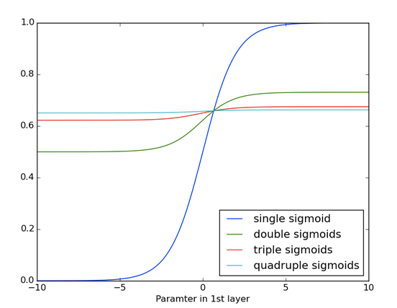
\includegraphics[width=0.9\linewidth]{images/vanishing_gradient}
	\caption{Vanishing Gradient Problem verdeutlicht an der Sigmoidfunktion \cite{deeplearning4j}} %Generelle
	\label{fig:vanishing}
\end{figure} 

So kann eine inkorrekte Vorhersage stattfinden. Aufgrund dessen wurden Long Short Term Memory-Netzwerke entwickelt, die zur Lösung des Problems beitragen. Dabei werden Recurrent Neural Networks mit einer Speicherstruktur erweitert, was zur Namensgebung führt. Diese Netzwerke sind in der Lage, anhand des Kontextes zukünftige Wörter vorherzusagen und so ihre Genauigkeit zu erhöhen. Auch beim Lernen und Erkennen verrauschter, geräuschverzerrter oder hallender Aufnahmen bzw. schlechten Bedingungen beim Bearbeiten der Merkmale kann diese Form von Netzwerken bessere Ergebnisse erzielen \cite{Yu.2014}. Die verbesserte Genauigkeit gegenüber gewöhnlichen tiefen neuronalen Netzen wird in verschiedenen Arbeiten belegt \cite{Yu.2014, 2015arXiv150706947S}. 
\\
Diese Form von Netzwerken erlauben die Erkennung von Mustern und Zusammenhängen zeitlich getrennter Ereignisse. Somit eignen sie sich um Zeitreihen zu verarbeiten und vorherzusagen. Sogar, wenn zwischen wichtigen Ereignissen Verzögerungen liegen, die eine unbekannte Länge aufweisen. 
Die grundsätzliche Idee dabei ist es über elementweise Multiplikationen den Informationsfluss in dem Netzwerk zu steuern. Eine LSTM-Zelle kann als intelligente Netzwerkeinheit betrachtet werden, welche Informationen über einen Zeitraum speichern kann. Dies wird durch eine Gating-Struktur erreicht. Die Information passiert verschiedene Gatter. Es wird bestimmt, wann es wichtig ist, sich an vorhergehende Eingaben zu erinnern, wann sich die Zelle Informationen weiter merken oder diese vergessen sollte und wann sie die Information ausgibt. Ein Gatter ist dabei nichts weiter, als eine Reihe von Multiplikationen bzw. Matrixoperationen {\cite{Yu.2014}}. 
Das System ist somit in der Lage aus dem Kontext heraus genaue Vorhersagen zu treffen, wodurch die Spracherkennung präziser wird. Eine Darstellung einer LSTM-Zelle ist Abbildung \ref{fig:lstm} zu sehen. Der Input x wird zur Zeit t von mehreren Quellen in die Zelle eingespeist. Dabei wird x an alle Gatter übergeben. Die Gatter i (Input), f (Forget), c (Memory cell), o (Output) und h (Hidden vector bzw. der resultierende Zustand) haben dabei ihre eigene Gewichtungsfunktion \cite{6638947}.   

\begin{figure}[h!]
	\centering
	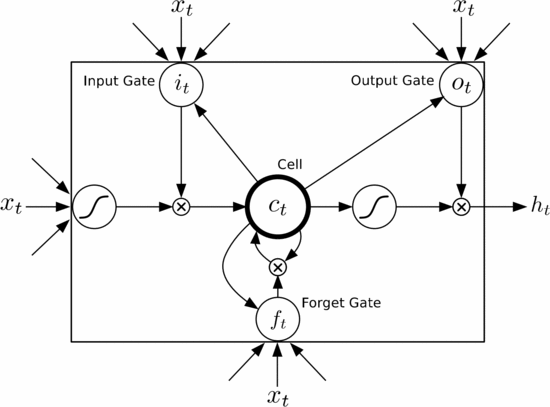
\includegraphics[width=0.9\linewidth]{images/lstm_cell}
	\caption{Modell einer LSTM-Zelle \cite{deeplearning4j}} %Generelle
	\label{fig:lstm}
\end{figure}  

Allerdings ist es selbst heute nicht möglich das Spracherkennungsproblem allgemein zu lösen. Spracherkennungssysteme werden somit nur für bestimmte Anwendungsfälle oder Szenarien konzipiert. Mit einer solchen Spezialisierung auf entsprechende Anwendungsgebiete können höhere Genauigkeiten erreicht werden. Zudem wird nicht so viel Rechenleistung und Speicher benötigt {\cite{beat_tobias}}. Vor allem bei der multilingualen Spracherkennung besteht die Schwierigkeit Gemeinsamkeiten verschiedener Sprachen zu nutzen, um Sprachen mit wenig Trainingsdaten mit einer ausreichenden Genauigkeit anzubieten. Es gilt die Sprachen zu finden, die zur besten Erkennungsleistung der neuen Sprache führen. Dabei müssen Beziehungen zwischen den Sprachen erkannt werden. Problematisch ist auch, dass gleiche Phoneme je nach Sprecher und Sprache variieren, was dazu führt, dass Phoneme nur im Kontext betrachtet werden (sogenannte Triphon-Zustände) {\cite{Yu.2014}}. Spracherkennungen verschiedener Unternehmen erreicht heute niedrige Wortfehlerraten (Google liegt bei 4,9\%), was auf die Menge von Trainingsmaterial zurückzuführen ist {\cite{venturebeat}} {\cite{9to5google}} {\cite{businessinsider}}. In der Literatur wird außerdem gezeigt, dass verschiedene Kombinationen von tiefen neuronalen Netzen und LSTM-Netzwerken zu einer weiteren Verbesserung führen {\cite{6638947}}. 